% Chapter 5
\usepackage{amsmath}
\usepackage{amsfonts}
\
\chapter{SYSTEM DEVELOPMENT} % Write in your own chapter
\section{MODULES USED}
\subsection{DATA PREPROCESSING}
JPEG uses a lossy image compression. Each re-encoding process (new saving) performed on the image leads to further loss of quality. The JPEG algorithm is based on a 8x8 pixel grid. Each 8x8 square grid is thereby treated and compressed separately. If the image is untouched, then all these 8x8 squares will show the same error level potential.  
\subsubsection{Algorithm:} 

1: The image is resaved with 95\%(or 90\%)JPEG quality.

2: Compare each(8*8) blocks of corresponding original and new resaved image. 

3: If image is unmodified , then all 8 x8 squares should have similar error potentials.

4: Else modified areas will appear with a higher potential error level . 

INPUT: Tampered image

OUTPUT: The output of ELA is image with higher error potential.

\subsection{TRAINING THE CNN}
\begin{figure}[htp]
\centering
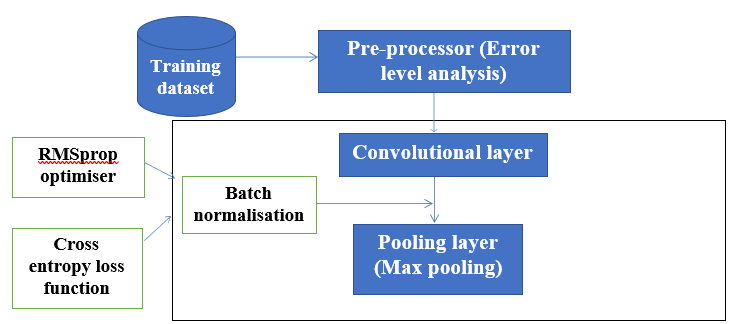
\includegraphics[scale=0.5,width=17cm]{Figures/training.png}
\caption{Training the model}
\label{fig:universe}
\end{figure}
The training process of a CNN is done through an iterative algorithm that alternates between feedforward  and back propagation passes of the data. The weights of the convolutional filters and fully-connected layers are updated at each iteration of the backpropagation passes. CNN is capable of learning classification features directly from the data. The ReLU activation function is applied to each value in the feature maps of every convolutional layer. The convolutional layers are followed by the max pooling layers. We use a batch normalization layer after each regular convolutional layer. However, the prediction error convolutional filters outputs are directly convolved with the next convolutional layer without using the batch normalization layer. We consider the RMSProp optimizer  to train our model. This module is proposed to extract features related to the traces left by different editing operations, and which are utilized to check the authenticity of images. 

INPUT: The pre-processed images 

OUTPUT: The trained classifier used to detect the tampered images. 

\subsubsection{Algorithm:} 
1.	Initialize w_k   using  randomly  drawn  weights

2.	i=1 

3.	while  i \leq  maximum\_iteration  do

4.	Do  feedforward  pass 

5.	Update filter weights through RMSProp optimizer and backpropagate errors 

6.	Set w_k(0, 0)^(^1^) = 0  for\tab all\tab K\tab filters 

7.	Normalize w_k^(^1^)  ’s  such  that  \Sigma_l_,_m_ \neq _0 w_k^(^1^)   (l, m) = 1 

8.	Set w_k(0, 0)^(^1^) = - 1   for  all  K  filters 

9.	i = i + 1 

10.	if training accuracy converges then

11.	exit 

12.	end 


\subsubsection{RMSPROP OPTIMISER }
The RMSprop optimizer is similar to the gradient descent algorithm with momentum. The RMSprop optimizer restricts the oscillations in the vertical direction. Therefore, we can increase our learning rate and our algorithm could take larger steps in the horizontal direction converging faster. 

              vdw =\beta. vdw  + (1- \beta).dw2  
                 
                     where  \beta is a momentum in learning rate 
              
              vdb  = \beta. vdw  + (1- \beta).db2
              
              W=W-\alpha dw/(\sqrt(v\_db )+∈)      
                     
                     where W weights to be updated during  backpropagation and  \alpha is a value always \textless 1.      
               
              b=b- \alpha dw/(\sqrt(v\_db )+\epsilon)     
              
                     where b is the calculated gradient, \epsilon is a small value added to prevent gradient from blowing up.

\subsubsection{CROSS ENTROPY LOSS FUNCTION}
Cross Entropy is commonly-used in binary classification (labels are assumed to take values 0 or 1) as a loss function (For multi-classification, use Multiclass Cross Entropy), which is computed by  

       L=-1/n \Sigma_(i_=_1)^n [\ (\ y^(^i^)  log(\ \^y^i)\ +(\ 1-y^i)log(\ 1-\^y^i) ]\
\newline  

Where L is a loss calculated which is the difference between the actual and the predicted output. 
Cross entropy measures the divergence between two probability distribution, if the cross entropy is large, which means that the difference between two distribution is large, while if the cross entropy is small, which means that two distribution is similar to each other.   
When the difference between predicted value and actual value is large, the learning speed, i.e., convergence speed, is fast, otherwise, the difference is small, the learning speed is small.  
Cross entropy cost function has the advantages of fast convergence and is more likely to reach the global optimization. 

\subsection{CLASSIFICATION BLOCK}
\begin{figure}[htp]
\centering
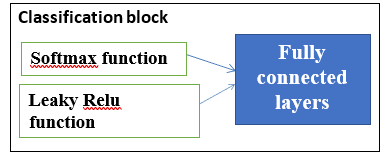
\includegraphics[scale=0.5,width=17cm]{Figures/classification.png}
\caption{Classification}
\label{fig:universe}
\end{figure}
This first layer of the classification block conatins about 256 nodes and accepts input as vectors. This layer uses ReLU activation function where negative values will not be considered significant hence makes it more efficient. To give the accurate result the last layer in the classification block of the neural network uses the softmax activation function which gives the highest activation level.The CNN model extracts the feature and classifies the pre-processed forged image to detect whether the given image is spiced or not.

\subsection{PASSIVE TYPE DETECTION}
Passive image authentication is a class of authentication techniques that uses the received image itself only for assessing its authenticity or integrity, without any side information (signature or watermark) of the original image from the sender.
This block is where the image that is not detected to be spliced is checked for copy move forgery using the following steps:

1.Blur image for eliminating image details

2.Convert image to degraded palette

3.Decompose the image into small NxN pixel blocks

4.Alphabetically order these blocks by their pixel values

5.Extract only these adjacent blocks which have small absolute color
difference

6.Cluster these blocks into clusters by intersection area among blocks

7.Extract only these clusters which are bigger than block size

8.Extract only these clusters which have similar cluster, by using some sort of similarity function (in this case Hausdorff distance between clusters)

9.Draw discovered similar clusters on image



